%! suppress = EscapeHashOutsideCommand
%! suppress = TooLargeSection
%! suppress = MissingLabel

% * Make friends tikz & colors
%   https://en.wikibooks.org/wiki/LaTeX/Colors
% * To enable vertical top alignment globally
%   https://tex.stackexchange.com/questions/9889/positioning-content-at-the-top-of-a-beamer-slide-by-default
\documentclass[usenames, dvipsnames]{beamer}
% ------------------------------------------------

% Graphics
\usepackage{color}
\usepackage{tabularx}
\usepackage{tikz}
\usepackage{blkarray}
\usepackage{graphicx}
% ------------------------------------------------

% Math
\usepackage{amsmath, amsfonts}
\usepackage{amssymb}
\usepackage{proof}
\usepackage{mathrsfs}
% Crossed-out symbols
% https://tex.stackexchange.com/questions/75525/how-to-write-crossed-out-math-in-latex
\usepackage[makeroom]{cancel}
\usepackage{mathtools}
% ------------------------------------------------

% Additional font sizes
% https://www.overleaf.com/learn/latex/Questions/How_do_I_adjust_the_font_size%3F
\usepackage{moresize}
% Additional colors
% https://www.overleaf.com/learn/latex/Using_colours_in_LaTeX
\usepackage{xcolor}
% ------------------------------------------------

% Language
\usepackage[utf8] {inputenc}
\usepackage[T2A] {fontenc}
\usepackage[english, russian] {babel}
\usepackage{indentfirst, verbatim}
\usetikzlibrary{cd, babel}
% ------------------------------------------------

% Fonts
\usepackage{stmaryrd}
\usepackage{cmbright}
\usepackage{wasysym}
% ------------------------------------------------

% Code
% https://tex.stackexchange.com/questions/99475/how-to-invoke-latex-with-the-shell-escape-flag-in-texstudio-former-texmakerx
\usepackage{minted}
\setminted{xleftmargin=\parindent, autogobble, escapeinside=\#\#}
% ------------------------------------------------

% Template
\usetheme{CambridgeUS}
\usecolortheme{dolphin}
% https://tex.stackexchange.com/questions/231439/beamer-how-to-make-font-larger-for-page-numbers
\setbeamerfont{headline}{size=\scriptsize}
\setbeamerfont{footline}{size=\scriptsize}
% Remove heddline
% https://tex.stackexchange.com/questions/33146/how-could-i-remove-a-header-in-a-beamer-presentation
%\setbeamertemplate{headline}{}
% Slide sizes
% https://tex.stackexchange.com/questions/56768/how-to-set-a-small-default-font-size-with-beamer
%\geometry{paperwidth=140mm,paperheight=105mm} % 4:3
\geometry{paperwidth=168mm,paperheight=105mm} % 16:10
% Remove navigation bar
% https://stackoverflow.com/questions/3210205/how-to-get-rid-of-navigation-bars-in-beamer
\beamertemplatenavigationsymbolsempty
% ------------------------------------------------

% Bullets
% https://9to5science.com/change-bullet-style-formatting-in-beamer
% https://tex.stackexchange.com/questions/185742/i-need-to-change-color-of-beamer-itemize-and-subitem-separately
\setbeamertemplate{itemize item}{\scriptsize\raise1.25pt\hbox{\donotcoloroutermaths$\blacktriangleright$}}
\setbeamertemplate{itemize subitem}{\tiny\raise1.5pt\hbox{\donotcoloroutermaths$\blacktriangleright$}}
\setbeamertemplate{itemize subsubitem}{\tiny\raise1.5pt\hbox{\donotcoloroutermaths$\blacktriangleright$}}
\setbeamertemplate{enumerate item}{\insertenumlabel.}
\setbeamertemplate{enumerate subitem}{\insertenumlabel.\insertsubenumlabel}
\setbeamertemplate{enumerate subsubitem}{\insertenumlabel.\insertsubenumlabel.\insertsubsubenumlabel}
% ------------------------------------------------

% Diff
\usepackage{multicol}
\usepackage{hyperref}
\usepackage{soul} % https://tex.stackexchange.com/questions/23711/strikethrough-text
% ------------------------------------------------

% Appendix
% Slide numbers
% https://tex.stackexchange.com/questions/70448/dont-count-backup-slides
\usepackage{appendixnumberbeamer}
\newcommand{\backupbegin}{
    \newcounter{framenumbervorappendix}
    \setcounter{framenumbervorappendix}{\value{framenumber}}
}
\newcommand{\backupend}{
    \addtocounter{framenumbervorappendix}{-\value{framenumber}}
    \addtocounter{framenumber}{\value{framenumbervorappendix}}
}
% ------------------------------------------------

% Custom commands
\newcommand{\err}[0]{\textcolor{red}{ошибка}}
% ------------------------------------------------

% Speaker notes
% https://tex.stackexchange.com/questions/114219/add-notes-to-latex-beamer
% https://tex.stackexchange.com/questions/35444/split-beamer-notes-across-multiple-notes-pages/35496#35496
%\setbeameroption{show notes on second screen=right} % enable speaker notes
%--------------------------------------

\author[Андрей Стоян]{Стоян Андрей Сергеевич \\ {\footnotesize научный руководитель: к.~ф.-м.~н.} Москвин Денис Николаевич \\ {\footnotesize научный консультант:} Новожилов Дмитрий Павлович}
\institute[ИТМО/SE]{Университет ИТМО\\Разработка программного обеспечения/Software engineering}

\title[Self-типы для языка Kotlin]{Дизайн и разработка Self-типов для языка Kotlin}
\date{Санкт-Петербург 2023г.}

\begin{document}
    \setcounter{framenumber}{-1}

    \maketitle


    \section{Введение}


    \subsection{Предметная область}

    \begin{frame}{Системы типов}
        \begin{itemize}
            \item Система типов позволяет выявлять заведомо некорректные программы путём классификации выражений по типам вычисляемых ими значений
            \item Проверка нетривиальных свойств программы --- неразрешимая задача
            \item Анализ типов отвергает много корректных программ, чтобы оставаться разрешимым
        \end{itemize}

        \begin{center}
            \includegraphics[width=0.36\textwidth]{fig/types}
        \end{center}

        \begin{block}{Задачи дизайна безопасной системы типов для промышленного языка программирования}
            \begin{itemize}
                \item Отвергнуть все некорректные программы (с точки зрения типов времени исполнения)
                \item Типизировать как можно больше корректных программ
                \item Сохранить практичность языка: сложность, количество необходимого рутинного кода
            \end{itemize}
        \end{block}
    \end{frame}


    \subsection{Постановка проблемы}

    \begin{frame}[fragile]{Ограничение текущей системы типов Kotlin}
        \vspace{-1em}
        \begin{columns}[onlytextwidth]
            \begin{column}[t]{0.5\textwidth}
                \begin{itemize}
                    \item Метод базового класса можно вызывать на объекте наследника
                    \item Нет прямого способа записать тип времени исполнения объекта, на котором вызывается метод (\emph{получателя вызова})
                \end{itemize}
                \begin{block}{Нехватка точности анализа типов}
                    \begin{itemize}
                        \item Семантика метода может гарантировать, что всегда возвращается объект того типа, на котором метод вызывается
                        \item Отвергаются корректные программы
                    \end{itemize}
                \end{block}
            \end{column}\hfill%
            \begin{column}[t]{0.460\textwidth}
                \begin{block}{Пример: персистентные коллекции}
                    \begin{minted}{kotlin}
                        interface PCollection<out E> {
                            fun add(x: T): #\framebox{PCollection<E>}#
                        }

                        interface PList<out E> :
                            PCollection<E> {
                            fun listSpecific()
                        }

                        fun test(xs: PList<Int>) {
                            xs.add(42) // : #\framebox{PCollection<T>}#
                              .listSpecific() // #\err#
                        }
                    \end{minted}
                \end{block}
            \end{column}
        \end{columns}
    \end{frame}

    \begin{frame}[fragile]{Другие случаи использования типа объекта получателя}
        \begin{block}{Пример: шаблон <<Наблюдатель>>}
            \begin{minted}{kotlin}
                val button = ConcreteButton()
                button.onClick { it: #\framebox{BaseButton}# -> /* ... */ }
            \end{minted}
        \end{block}
        \begin{block}{Пример: алгебры}
            \begin{minted}{kotlin}
                interface Semigroup {
                    fun combine(other: #\framebox{Semigroup}#): #\framebox{Semigroup}#
                }
            \end{minted}
        \end{block}

        \begin{block}{Нехватка полноты анализа типов}
            \begin{itemize}
                \item Семантика метода может на вход требовать тот же тип, на котором метод вызывается
                \item Система типов не может гарантировать выполнение этого инварианта
            \end{itemize}
        \end{block}
    \end{frame}


    \subsection{Существующие решения}

    \begin{frame}[fragile]{Дополнительный типовой параметр}
        \begin{block}{Пример: персистентные коллекции с дополнительным типовым параметром}
            \begin{minted}[escapeinside=??]{kotlin}
                interface PCollection<out E, ?\framebox{out S : PCollection<E, S>}?> {
                    fun add(value: E): ?\framebox{S}?
                }
                interface PList<out E, ?\framebox{out S : PList<E, S>}?> : PCollection<E, ?\framebox{S}?> {
                    fun listSpecific()
                }
                fun <?\framebox{L : PList<Int, L>}?> test(xs: ?\framebox{L}?) {
                    xs.add(42) /* : ?\framebox{L}? */ .listSpecific()
                }
            \end{minted}
        \end{block}

        \begin{block}{Недостатки}
            \begin{itemize}
                \item Паттерн рекурсивного ограничения распространяется по всему коду
                \item Требуется явное приведение типов: \mintinline[escapeinside=??]{kotlin}|this as S|
                \item Однажды зафиксированный типовой аргумент \texttt{S} не может быть уточнён в наследниках
            \end{itemize}
        \end{block}
    \end{frame}

    \begin{frame}[fragile]{Добавление abstract override методов}
        \begin{block}{Пример: персистентные коллекции с abstract override методами}
            \begin{minted}[escapeinside=??]{kotlin}
                interface PCollection<out E> {
                    fun add(value: E): ?\framebox{PCollection<E>}?
                }
                interface PList<out E> : PCollection<E> {
                    abstract override fun add(value: E): ?\framebox{PList<E>}?
                    fun listSpecific()
                }
                fun test(xs: PList<Int>) {
                    xs.add(42) /* : ?\framebox{PList<Int>}? */ .listSpecific()
                }
            \end{minted}
        \end{block}

        \begin{block}{Недостатки}
            \begin{itemize}
                \item Много рутинного кода: переопределить каждый метод в каждом наследнике
                \item Нет контроля компилятора, что abstract override методы не были забыты
                \item Работает только для возвращаемого типа (типы параметров обязаны совпадать)
            \end{itemize}
        \end{block}
    \end{frame}

    \begin{frame}[fragile]{Self-типы}
        \begin{itemize}
            \item Вводится специальный тип \texttt{Self} (или \texttt{ThisType} в литературе)
            \item \texttt{Self} ссылается на тип наследника, на котором вызывается метод (тип получателя)
            \item \texttt{Self} --- тип специального параметра \mintinline{kotlin}|this| (объекта получателя вызова)
            \item Подход не имеет упомянутых ранее недостатков
        \end{itemize}

        \begin{block}{Пример: персистентные коллекции с Self-типами}
            \begin{minted}[escapeinside=??]{kotlin}
                interface PCollection<out E> {
                    fun add(value: E): ?\framebox{Self}?
                }
                interface PList<out E> : PCollection<E> {
                    fun listSpecific()
                }
                fun test(xs: PList<Int>) {
                    xs.add(x) /* : ?\framebox{PList<Int>}? */ .listSpecific()
                }
            \end{minted}
        \end{block}
    \end{frame}


    \section{Цель и задачи}

    \begin{frame}{Цель и задачи}
        \begin{block}{Цель}
            Разработать дизайн Self-типов для языка Kotlin на основании опыта других языков и реализовать поддержку Self-типов в компиляторе kotlinc.
        \end{block}

        \begin{block}{Задачи}
            \begin{enumerate}
                \item Выделить особенности существующих решений: возможные значения Self-типа, допустимые позиции Self-типа и меры по обеспечению безопасности системы типов
                \item Интегрировать Self-типы в типовую систему языка Kotlin на основании проведённого анализа решений
                \item Реализовать поддержку Self-типов в компиляторе kotlinc
            \end{enumerate}
        \end{block}
    \end{frame}


    \section{Ход работы}


    \subsection{Существующие решения}

    \begin{frame}{Обзор существующих решений}
        \begin{block}{Академические подходы}
            \begin{itemize}
                \item Объекты, классы и их типы кодируются в типизированном лямбда-исчислении с записями, подтипизацией, экзистенциальными и рекурсивными типами
                \item На простой модели видны потенциальные возможности сделать систему небезопасной
                \item Предлагаются наиболее гибкие решения, как правило, в ущерб простоте
                \item Свойства результатов доказываются на модельных исчислениях [\href{https://dl.acm.org/doi/pdf/10.1145/503502.503505}{FJ}, \href{https://dl.acm.org/doi/pdf/10.1145/2888392}{CoreThisJava}]
            \end{itemize}
        \end{block}

        \begin{block}{Прикладные языки, поддерживющие Self-типы}
            \begin{itemize}
                \item $\color{red} \mathbf{\times}$ Python, TypeScript, Java с плагином Manifold --- небезопасная реализация
                \item $\color{red} \mathbf{\times}$ Rust --- запрещено создавать трейт-объект\footnote{Трейты --- механизм специального полиморфизма в Rust}\footnote{Трейт-объект --- способ использовать неизвестный тип, реализующий трейт: \mintinline{rust}|Box<dyn Trait>|} при наличии метода с Self-типом
                \item Swift --- безопасная реализация Self-типов
            \end{itemize}
        \end{block}
    \end{frame}


    \subsection{Интеграция Self-типов в типовую систему языка Kotlin}

    \begin{frame}[fragile]{Материализация Self-типа}
        \vspace{-1em}
        \begin{columns}[onlytextwidth]
            \begin{column}[t]{0.485\textwidth}
                \begin{block}{Пример: небезопасность покидания Self-типом контекста объекта}
                    \begin{minted}{kotlin}
                        abstract class A {
                            fun self(): Self = this
                            fun unsafe(a: A): Self = #\framebox{a.self()}#
                        }

                        class B : A() {
                            fun bOnly() {}
                        }

                        fun test(a: A, b: B) {
                            b.unsafe(a) // область видимости B
                             .bOnly()   // #\err#
                        }
                    \end{minted}
                \end{block}
            \end{column}\hfill%
            \begin{column}[t]{0.485\textwidth}
                \begin{block}{Теоретическое решение}
                    Чтобы воспользоваться содержимым рекурсивного типа $\mu Self\ldotp T[Self]$ требуется воспользоваться правилом развёртки:
                    \begin{equation*}
                        %! suppress = EscapeAmpersand
                        \infer[\text{Unfold}]{
                            \Delta \vdash unfold(o) : [Self \mapsto U]T
                        }{
                            U = \mu Self \ldotp T & \Delta \vdash o : U
                        }
                    \end{equation*}
                \end{block}
                \begin{block}{Решение для Kotlin}
                    \begin{itemize}
                        \item Self-тип должен переписываться в тип получателя в его области видимости:
                        \[(self : A.() \to \framebox{$A$}) \in scope(A)\]
                        \item Ограничение подтипизации: \[\forall T \ldotp T \bcancel{<:} Self\]
                    \end{itemize}
                \end{block}
            \end{column}
        \end{columns}
    \end{frame}

    \begin{frame}{Значения Self-типа: существующие решения}
        \begin{block}{Академические решения}
            \begin{itemize}
                \item Вводятся специальные виды методов, в которых новые объекты могут иметь Self-тип
                \item Усложняется разработка компилятора и затрудняется последующее развитие языка
                \item Ненаследуемые методы [\href{http://www.fos.kuis.kyoto-u.ac.jp/~igarashi/papers/pdf/thistype-SAC09.pdf}{Saito et al, 2009}]
                \begin{itemize}
                    \item Не могут быть унаследованы --- требуется переопределение в каждом наследнике
                \end{itemize}
                \item Виртуальные конструкторы [\href{https://www.researchgate.net/profile/Sukyoung-Ryu/publication/254004584_Exact_type_parameterization_and_ThisType_support/links/54b90ed10cf269d8cbf72d01/Exact-type-parameterization-and-ThisType-support.pdf}{Na et al, 2012}]
                \begin{itemize}
                    \item Специальный метод может быть унаследован при выполнении набора ограничений
                \end{itemize}
            \end{itemize}
        \end{block}

        \begin{block}{Решения в прикладных языках}
            \begin{itemize}
                \item Только объект получатель (\mintinline{kotlin}|this|/\mintinline{swift}|self|) имеет Self-тип
                \item Не поддерживается возможность создания новых объектов Self-типа
                \item Хотя это необходимо для важных приложений (например, персистентных коллекций)
            \end{itemize}
        \end{block}
    \end{frame}

    \begin{frame}[fragile]{Значения Self-типа: Kotlin}
        \vspace{-1em}
        \begin{columns}[onlytextwidth]
            \begin{column}[t]{0.485\textwidth}
                \begin{block}{Условие замены типа \texttt{C} на \texttt{Self}}
                    \mintinline{kotlin}|C::class isSubtypeOf this.getClass()|\footnote{Условие должно выполняться всегда и быть проверяемо статически}
                \end{block}
                \begin{block}{Правило значений Self-типа для Kotlin}
                    \begin{enumerate}
                        \item Класс \texttt{C} должен быть финальным
                        \item Тип \mintinline{kotlin}|this@decl|
%                        \footnote{Получатель вызова текущей декларации}
                        либо равен \texttt{С}, либо включает \texttt{C} после smart-cast
                        \item Тип \texttt{C} объявлен в том же модуле, в котором создаётся объект
%                        \footnote{Иначе открытие класса нарушало бы совместимость исходных кодов}
                    \end{enumerate}
                \end{block}
            \end{column}\hfill%
            \begin{column}[t]{0.485\textwidth}
                \begin{block}{Пример: неизменяемая структура данных}
                    \begin{minted}[escapeinside=??]{kotlin}
                        sealed interface Data {
                            data class One(val a: Int) : Data

                            data class Two(
                                val a: Int, val b: Int
                            ) : Data

                            fun update(a: Int): Self =
                                when (this) {
                                    is One -> ?\colorbox{green}{One(a)}?
                                    is Two -> ?\colorbox{green}{Two(a, b)}?
                                }
                        }
                    \end{minted}
                \end{block}
            \end{column}
        \end{columns}
    \end{frame}

    \begin{frame}[fragile]{Ковариантные позиции Self-типа}
        \begin{block}{Ковариантные позиции}
            Позиции типов значений, предоставляемых методом вызывающему коду.
            Примеры:
            \begin{itemize}
                \item \mintinline{kotlin}|fun add(): #\framebox{Self}#| из \mintinline{kotlin}|interface PCollection<out E>|
                \item \mintinline{kotlin}|fun onClick(observer: (#\framebox{Self}#) -> Unit)| из \mintinline{kotlin}|abstract class BaseButton|
            \end{itemize}
        \end{block}

        \begin{block}{Академические результаты}
            \begin{itemize}
                \item Self-типы можно безопасно использовать в произвольной ковариантной позиции
            \end{itemize}
        \end{block}

        \begin{block}{Решение в Swift}
            \begin{itemize}
                \item В языке нет поддержки вариантности типовых параметров
                \item Полностью разрешена только позиция возвращаемого типа
            \end{itemize}
        \end{block}

        \begin{block}{Решение для Kotlin}
            \begin{itemize}
                \item Есть поддержка вариантности типовых параметров
                \item Допустимо использовать Self-типы во всех ковариантных позициях
            \end{itemize}
        \end{block}
    \end{frame}

    \begin{frame}[fragile]{Контравариантные позиции Self-типа: существующие решения}
        \begin{block}{Контравариантные позиции}
            Позиции типов значений, получаемых реализацией метода.
            Пример:
            \begin{itemize}
                \item \mintinline{kotlin}|fun combine(other: #\framebox{Self}#): Self| из \mintinline{kotlin}|interface Semigroup|
            \end{itemize}
        \end{block}

        \begin{block}{Академические результаты}
            \begin{itemize}
                \item При наличии Self-типа в контравариантной позиции наследник не является подтипом~[\href{https://dl.acm.org/doi/pdf/10.1145/96709.96721}{Cook et al, 1989}], назовём соответствующие методы \emph{сложными}
                \item Для поддержания сложных методов вводятся массивные изменения в системе типов
                \begin{itemize}
                    \item Отношение matching'а вместо подтипизации [\href{https://www.researchgate.net/profile/Kim-Bruce-2/publication/221496196_Subtyping_Is_Not_a_Good_Match_for_Object-Oriented_Languages/links/09e415122545c6d7a4000000/Subtyping-Is-Not-a-Good-Match-for-Object-Oriented-Languages.pdf}{Bruce et al, 1996}]
                    \item Разделение точных и экзистенциальных типов, локальное уточнение [\href{https://citeseerx.ist.psu.edu/document?repid=rep1&type=pdf&doi=a9d601d3bf8c921748902d58078d0a1b28f6ec4d}{Saito et al, 2009}]
%                    \item Именованные wildcard'ы и точные типовые параметры [\href{https://www.researchgate.net/profile/Sukyoung-Ryu/publication/254004584_Exact_type_parameterization_and_ThisType_support/links/54b90ed10cf269d8cbf72d01/Exact-type-parameterization-and-ThisType-support.pdf}{Na et al, 2012}]
                \end{itemize}
            \end{itemize}
        \end{block}

        \begin{block}{Решение в Swift}
            \begin{itemize}
                \item На экзистенциальных типах\footnote{Экзистенциальный тип в Swift --- неизвестный тип, реализующий протокол: \mintinline{swift}|any Protocol|} запрещено вызывать сложные методы
                \item В классах Self-типы в контравариантной позиции запрещены
            \end{itemize}
        \end{block}
    \end{frame}

    \begin{frame}[fragile]{Контравариантные позиции Self-типа: решение для Kotlin}
        \begin{itemize}
            \item Существующие решения запрещают виртуальную диспетчеризацию на сложных методах
            \item Заменим виртуальную диспетчеризацию статической с помощью эмуляции трейтов
            \item Нет необходимости поддерживать Self-типы в контравариантных позициях в Kotlin
        \end{itemize}

        \begin{block}{Эмуляция трейтов с помощью контекстов языка Kotlin}
            \begin{minted}{kotlin}
                interface Semigroup<S> {
                    fun S.combine(other: S): S
                }

                context(Semigroup<S>)
                fun <S> combineAll(xs: Iterable<S>): S =
                    xs.reduce { acc, x -> acc.combine(x) }
            \end{minted}
        \end{block}
    \end{frame}


    \subsection{Реализация поддержки Self-типов в компиляторе kotlinc}

    \begin{frame}{Детали реализации Self-типов в компиляторе kotlinc}
        \begin{enumerate}
%            \item Идентификатор типа \texttt{Self} введён как ключевое слово языка
%            \item Введён новый вид типов --- Self-типы
            \item Правила системы типов Kotlin доопределены для работы с Self-типами:
            \begin{itemize}
                \item Правило подтипизации
                \item Правило определения непосредственных супертипов
                \item Правило вычисления ближайших общих супертипов
            \end{itemize}
            \item Реализована материализация Self-типов в областях видимости\footnote{Области видимости --- сервисы компилятора, возвращающие множество функций, для которых объект данного типа может быть использован как получатель: $(plus : String\ldotp(String) \to String) \in scope(String)$}
            \begin{itemize}
                \item Для каждого места вызова метода с Self-типом генерируется синтетическая декларация
                \item В будущем потребуется разработать более эффективную реализацию
            \end{itemize}
%            \item Реализовано преобразование, подменяющее Self-тип на его границу и метаинформацию, при переходе к промежуточному представлению бекенда компилятора (IR)
            \item Полученная реализация протестирована на предмет допуска кода валидных сценариев использования и отвержения небезопасного кода % TODO N десятков тестов
        \end{enumerate}
    \end{frame}

    \begin{frame}{Функциональное тестирование}
        \begin{block}{Поддержка ковариантных позиций}
            TODO % TODO
        \end{block}
        \begin{block}{Поддержка типизации посторонних объектов Self-типом}
            TODO % TODO
        \end{block}
        \begin{block}{Проверка на использование Self-типов в недопустимых позициях}
            TODO % TODO
        \end{block}
    \end{frame}


    \section{Результаты}

    \begin{frame}{Результаты}
        \begin{enumerate}
            \item Проанализированы существующие реализации Self-типов в других языках на предмет их возможностей и мер по обеспечению безопасности системы с Self-типами
            \item Self-типы интегрированы\footnote{\url{https://github.com/winter-yuki/kotlin-self-types}} в типовую систему языка Kotlin с опорой на существующие решения
            \item Поддержка Self-типов реализована\footnote{\url{https://github.com/winter-yuki/kotlin/tree/self-types}} в компиляторе kotlinc за счет добавления специального вида типов и материализации Self-типов в областях видимости
        \end{enumerate}
    \end{frame}


    \appendix


    \section{Дополнительные слайды}

    \begin{frame}{}
        TODO % TODO
    \end{frame}

\end{document}
